\section{Results and discussion}
\label{sec:results}

Realizados los experimentos, la \tablename $.$\ref{tabla2} muestra los $RMSE$ obtenidos, en la cual se puede observar que las ESN obtienen un resultado muy diferente a las demás técnicas. El $RMSE$ promedio obtenido por las ESN $11085.47$ es cercano a 20 veces el de las otras técnicas. Este resultado de las ESN se explica debido a que estas redes neuronales recurrentes parten de estados aleatorios para irse ajustando en el proceso de entrenamiento, y por tanto, los valores obtenidos son reflejo de que la cantidad de datos disponibles no logra que la red neuronal se ajuste.
%
\begin{table}[h] 
\caption{Promedio y desviación estándar de los RMSE obtenidos por Finca} 
\label{tabla2} 
\centering
\begin{tabular}{c|c|c|c} 
\hline
\bfseries Farm & \bfseries Technique & \bfseries $RMSE_mean$ & \bfseries $RMSE_std$\\ 
\hline\hline 
28 Millas  	& Elastic net  & 463.56	& 	82.39  \\
			& SVR with linear kernel  & 465.92  & 85.70  \\
			& SVR with Gaussian kernel  & 466.63 & 89.53  \\						
			& Linear regression  & 468.25 & 83.57  \\									
			& SVR with sigmoid kernel & 552.81 & 123.82  \\									
			& ESN  & 11085.47 &  7965.66 \\												
\hline 
La Rita  	& SVR with linear kernel  & 816.29	& 	216.43  \\
			& Elastic net   &  817.98 &  211.14 \\
			& SVR with Gaussian kernel  & 820.92 & 231.21  \\						
			& Linear regression  & 823.55 &  213.24 \\									
			& SVR with sigmoid kernel & 1070.58 &  331.89 \\									
			& ESN  & 8329.72 & 5435.54  \\												
\hline    
\end{tabular} 
\end{table}
%
Adicionalmente, la \figref{figura4} muestra los box plots con respecto a los $RMSE$ obtenidos. Se grafica ESN por separado debido a la diferencia de escala. Con respecto a las otras técnicas, la regresión lineal, Elastic net, SVR with gaussian kernel y SVR with linear kernel presentan compartamientos muy similares y aunque el promedio del $RMSE$ es diferente entre las fincas, La Rita cercano a 450 y 28 Millas cercano a 820, el comportaniento relativo de las técnicas es el mismo. Por su parte, SVR with sigmoid kernel presenta un promedio de $RMSE$ muy inferior a ESN, pero superior a las otras cuatro técnicas.
%
\begin{figure}[H] 
 \centering
 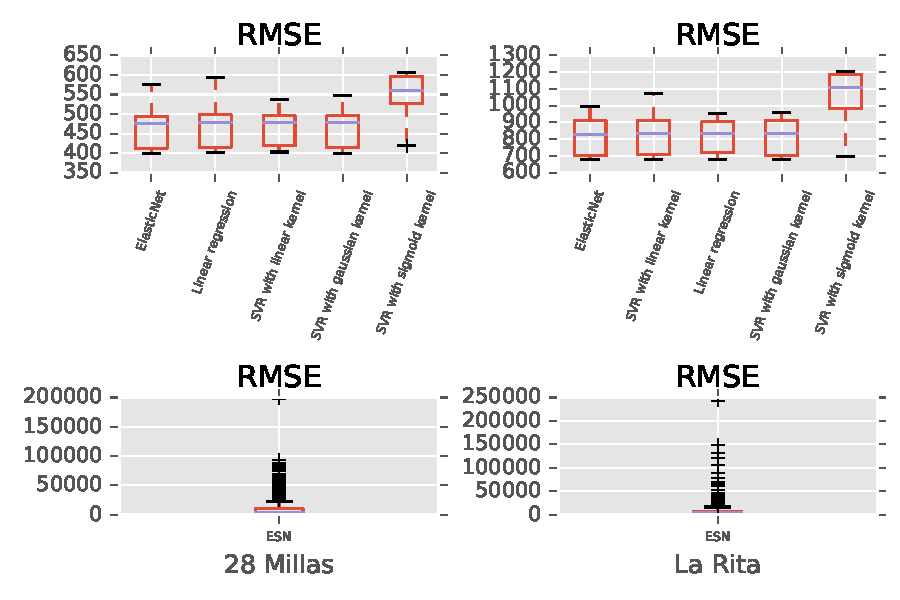
\includegraphics[width=1.0\linewidth]{Usado_2017-04-30_Sigatoka_RMSE_Boxplot_4}
 \caption{Box plots de los RMSE para cada una de las Fincas} 
 \label{figura4} 
\end{figure}
%
\figref{figura5} shows the Pareto frontier for each farm with respect to $R^2$ and $RMSE$. The red dots correspond to the observations belonging to Pareto frontier. La Rita obtains upper $R^2$ with respect to 28 Millas, but 28 Millas obtains better $RMSE$ than La Rita. This situation arise because $RMSE$ considers errors only with respect the prediction and in 28 Millas the average of Stage of Evolution is $4316.16$, unlike, in La Rita the average is $5507.30$. So, in La Rita we obtains higher errors in absolute values. $R^2$  is a relative metric between 0 thru 1 and it is less sensitive to absolute values.
%
\begin{figure}[H] 
 \centering
 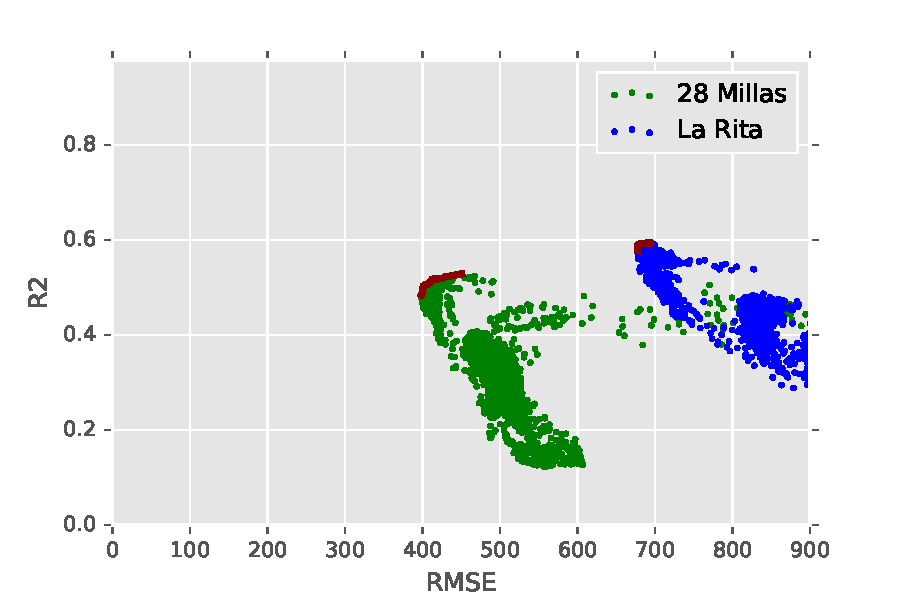
\includegraphics[width=1.0\linewidth]{Usado_2017-04-30_Sigatoka_R2_RMSE}
 \caption{Pareto frontier for $R^2$ and $RMSE$} 
 \label{figura5} 
\end{figure}

The Pareto frontier for the La Rita farm is composed by 5 elements. The \tablename $.$\ref{tabla3} shows the composition about variables, observation ranges, techniques and weeks ahead.

\begin{table}[h] 
\caption{Composition of the Pareto frontier - La Rita} 
\label{tabla3} 
\centering
\begin{tabular}{c|c|c|c|c|c} 
\hline
\bfseries Variable & \bfseries Observation  & \bfseries Weeks & \bfseries Technique &\bfseries $RMSE$ & \bfseries $R^2$\\ 
                   & \bfseries range - weeks & \bfseries ahead   & & & \\
\hline\hline 
$\overline{T}_{a}$ $\overline{W}$ &	1  & 1 & SVR with linear kernel & 693.39 & 59.4\% \\
										&	2  & 1 & SVR with linear kernel & 683.22 & 59.4\% \\
\hline 
$\overline{T}_{a}$  &  5 & 1 &  SVR with linear kernel & 679.25 & 59.2\% \\
\hline 
$\overline{T}_{a}$ $\overline{H}$ &	5  & 1 & Elastic net & 677.49 & 57.8\% \\
										&	5  & 1 & SVR with linear kernel & 677.37 & 59.1\% \\
\hline										
\end{tabular} 
\end{table}
%
Similarly, the Pareto frontier for the 28 Millas farm is composed by 15 elements. The \tablename $.$\ref{tabla4} shows the composition about variables and observation ranges.

\begin{table}[h] 
\caption{Composition of the Pareto frontier - 28 Millas} 
\label{tabla4} 
\centering
\begin{tabular}{c|c|c|c|c|c} 
\hline
\bfseries Variable & \bfseries Observation  & \bfseries Weeks & \bfseries Technique &\bfseries $RMSE$ & \bfseries $R^2$\\ 
                   & \bfseries range - weeks & \bfseries ahead   & & & \\
\hline\hline 
$\overline{T}_{a}$ $\overline{H}$ $\overline{W}$ $P$  &	9  & 1  & Elastic net & 398.65 & 48.5\% \\
													&	8  & 1 & Elastic net & 399.57 & 48.8\% \\
													&	7  & 1 & Elastic net & 399.65 & 49.1\% \\													
\hline 													
$\overline{T}_{a}$ $\overline{H}$ $\overline{W}$  &	9  & 1  & SVR with linear kernel & 399.86 & 49.3\% \\
												&	7  & 1  & SVR with linear kernel & 400.87 & 50.3\% \\
												&	6  & 1  & SVR with linear kernel & 403.40 & 50.7\% \\
												&	3  & 1  & SVR with gaussian kernel & 407.25 & 90.7\% \\													
\hline 													
$\overline{T}_{a}$ $\overline{H}$  &	4  & 1  & Elastic net & 400.65 & 49.6\% \\
									&	1  & 1  & SVR with linear kernel & 412.26 & 51.8\% \\
									&	2  & 1  & SVR with linear kernel & 409.18 & 51.2\% \\			
\hline 																												
$\overline{T}_{a}$ $\overline{H}$ $P$  & 2  & 1  & SVR with linear kernel & 410.71 & 51.2\% \\
\hline 																												
All  & 7  & 1  & SVR with linear kernel & 426.19 & 51.9\% \\
     & 5  & 1  & SVR with linear kernel & 428.66 & 52.3\% \\
     & 5 & 1  & Elastic net & 433.03 & 52.4\% \\
     &  5 & 1  & Linear regression & 450.48 & 53.0\% \\          
\hline	
\end{tabular} 
\end{table}
%
Now, the \figref{figura6} compares the mean of the $RMSE$ for each technique in the experiment. Se muestra el $RMSE$ para la predicción de 1, 2 ó 3 semanas adelante con respecto a la información de las variables climatológicas y del preaviso biológico observadas. Se aprecia que to predict one week ahead obtiene un $RMSE$ más bajo que two weeks ahead, and this is lower than three weeks ahead, lo cual es lo esperado pues entre más semanas adelante se desee predecir (en el futuro), hay más incertidumbre.
%
\begin{figure}[H] 
 \centering
 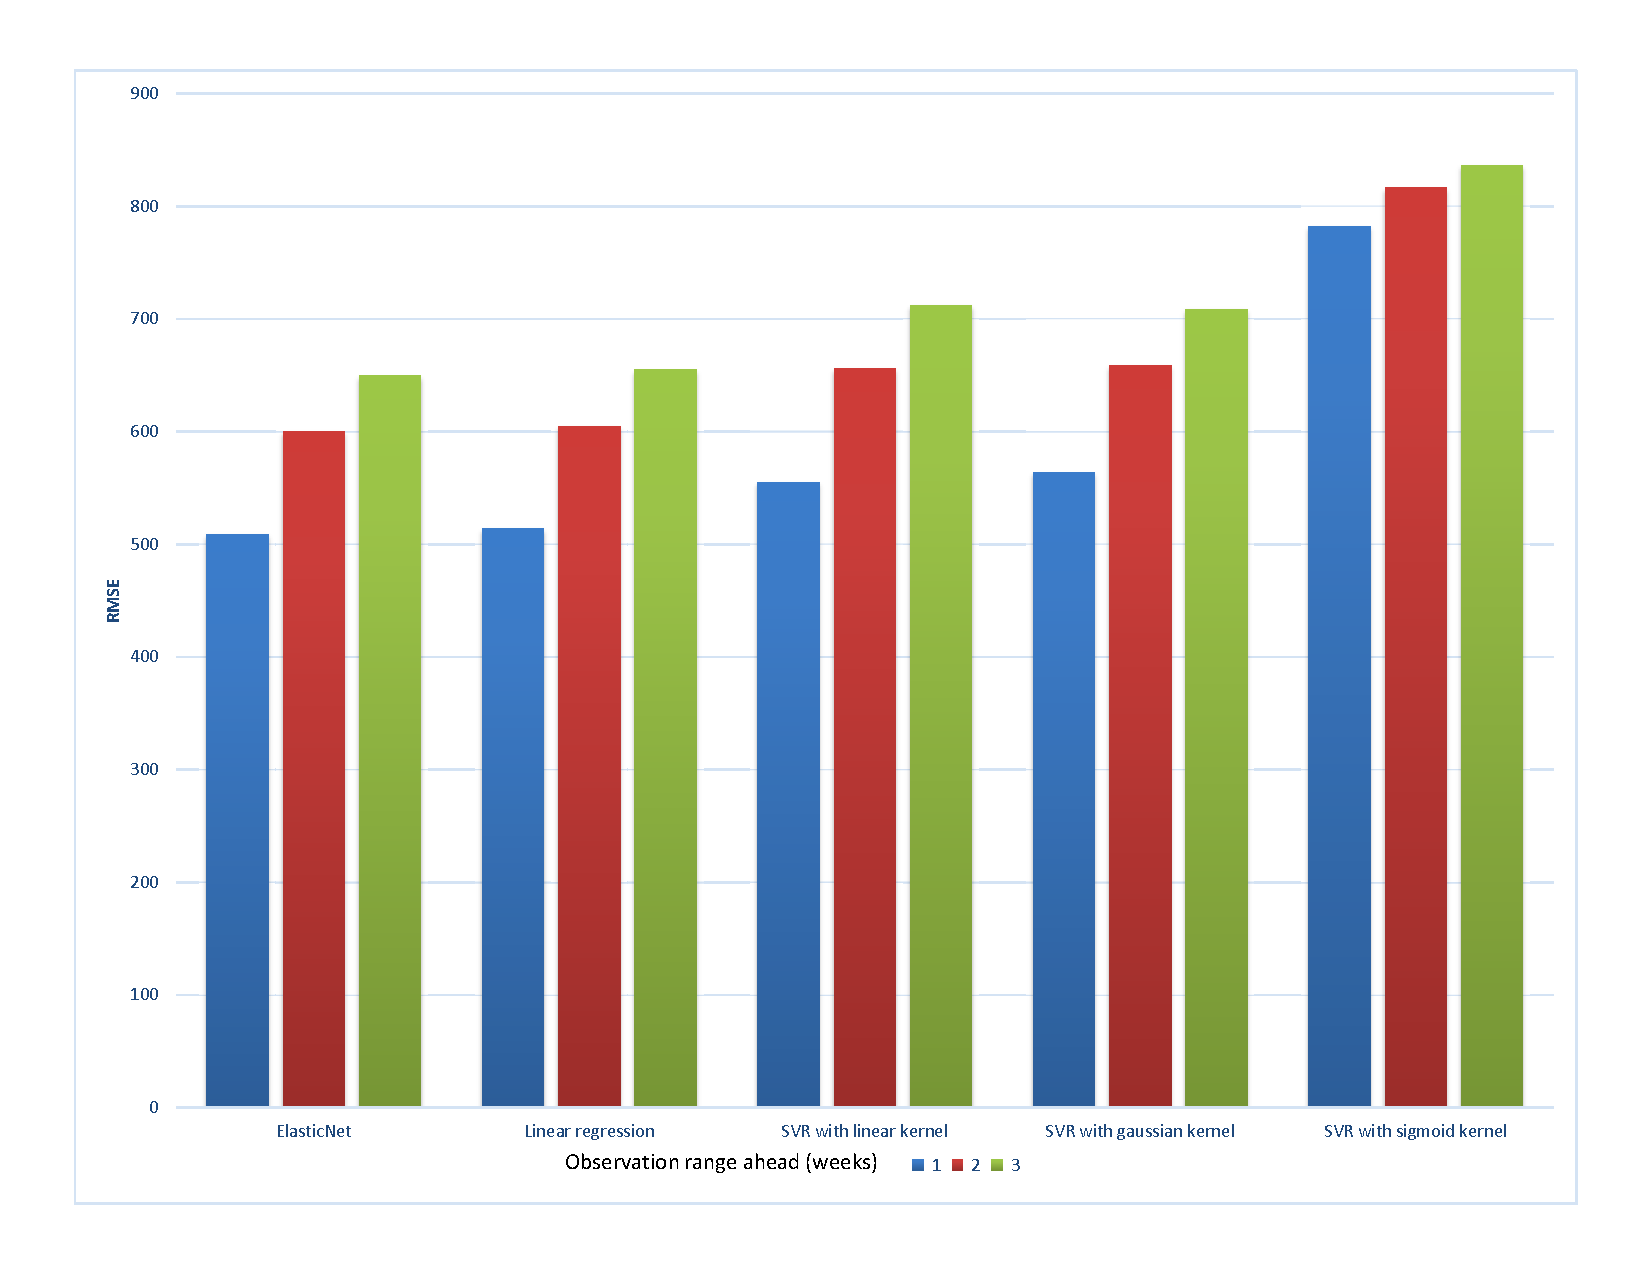
\includegraphics[width=1.0\linewidth]{Usado_Algorithms-RMSE}
 \caption{$RMSE$ for each algorithm} 
 \label{figura6} 
\end{figure}
%
\figref{figura7} shows the the mean $RMSE$ for each variables combination. The better results are obtained with $\overline{T}_{a}$, $\overline{W}$ and $P$.  Incluir más variables en el modelo no asegura mejorar la métrica, lo cual es importante pues este resultado sugiere que the use of more sensors do not assure a better result of prediction. 
%
\begin{figure}[H] 
 \centering
 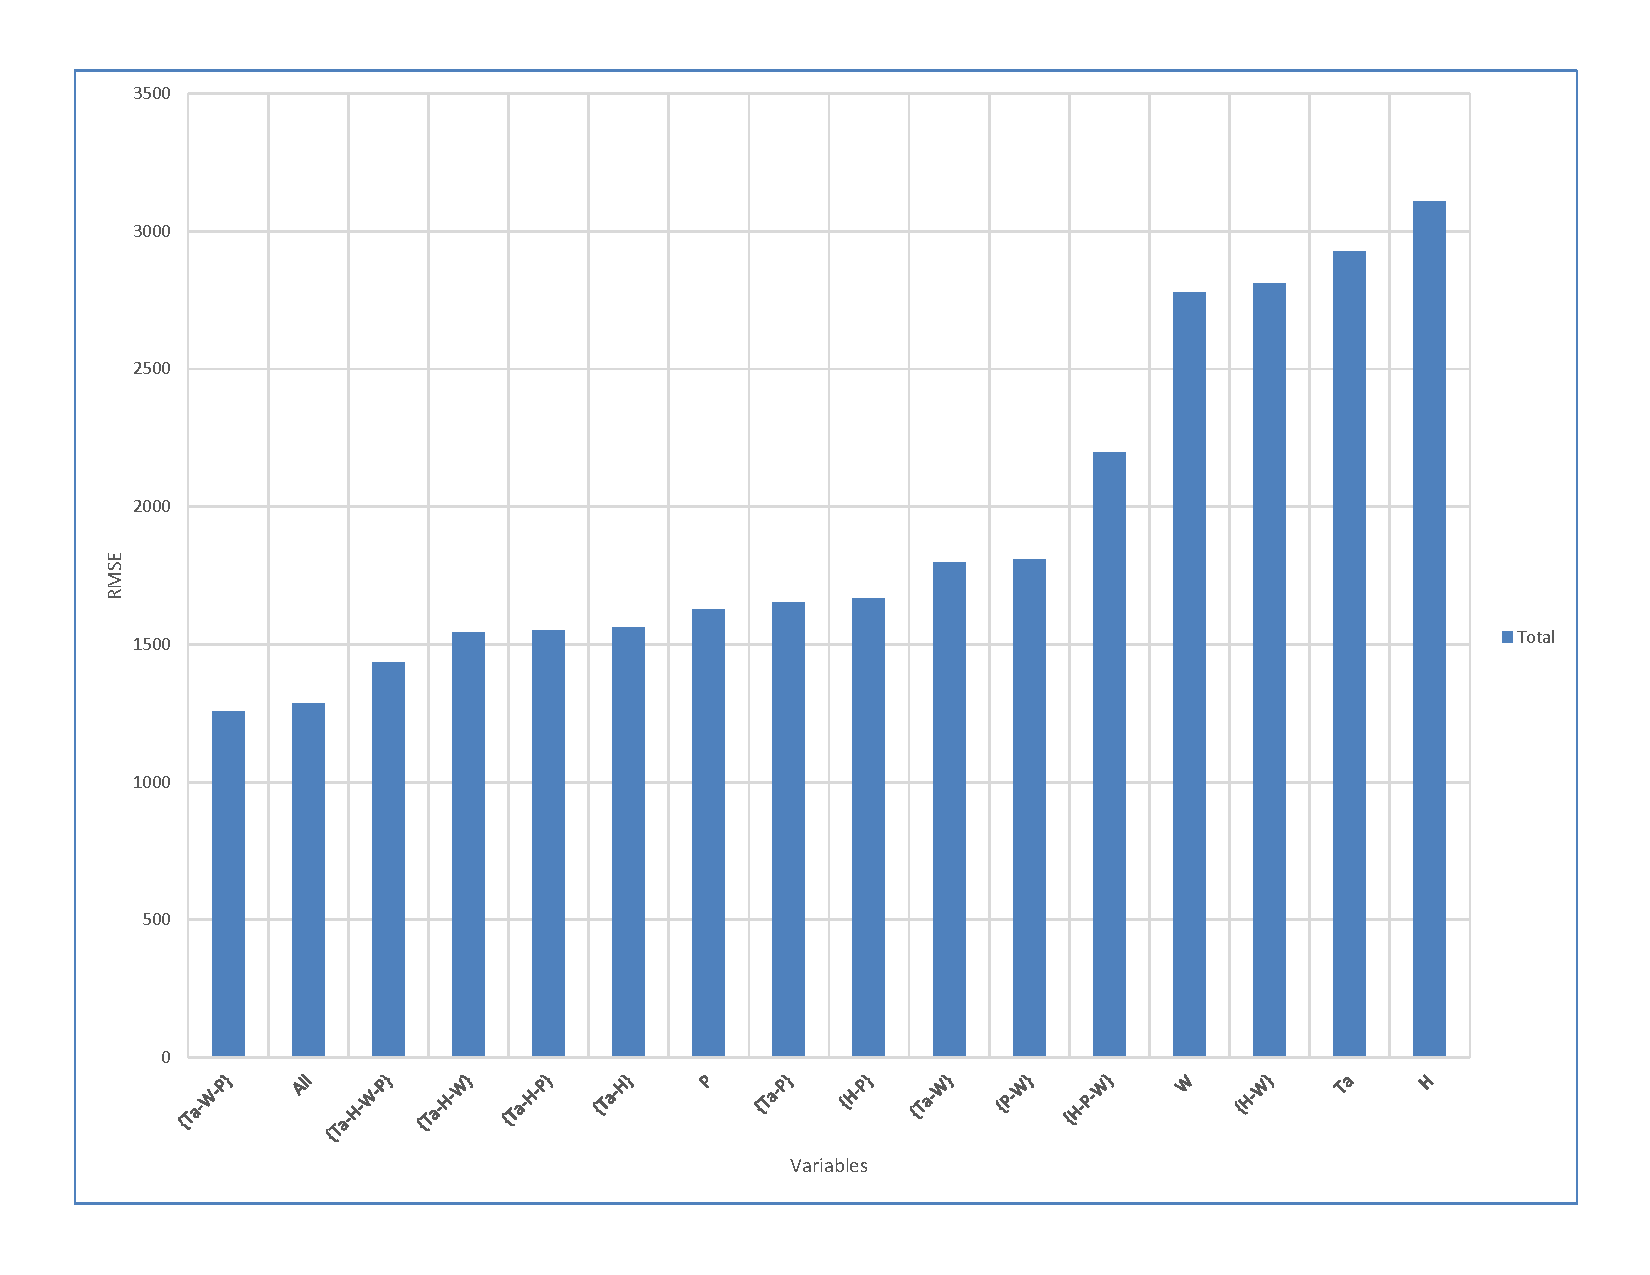
\includegraphics[width=1.0\linewidth]{Usado_Variables-RMSE}
 \caption{$RMSE$ for each variable combination} 
 \label{figura7} 
\end{figure}
%


